

向如此小的解决方案添加测试并不是非常具有挑战性。真正的困难来自于高级和较长的程序。多年来,我发现当我的代码接近1000行时,慢慢地就很难跟踪哪些行和分支在测试期间执行了,哪些没有执行。跨越3000行之后,这几乎是不可能的。大多数专业应用程序的代码都比这多得多。为了处理这个问题,可以使用一个实用工具来理解测试用例“覆盖”了哪些代码行。这样的代码覆盖工具与SUT挂钩,并在测试期间收集关于每一行执行的信息,以便将其显示在一个方便的报告中:

\begin{center}
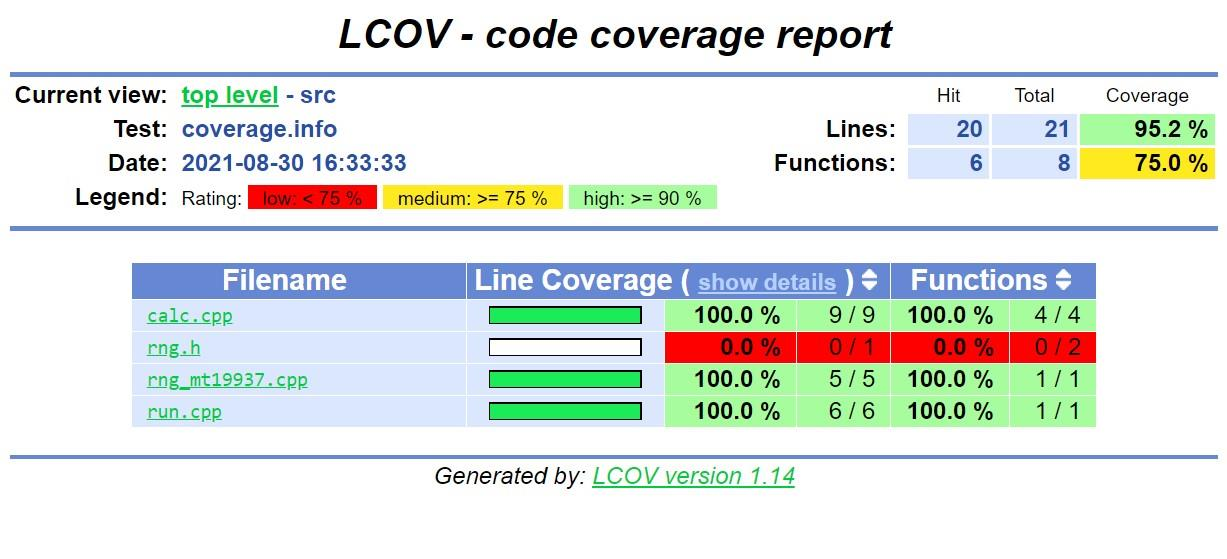
\includegraphics[width=0.8\textwidth]{content/3/chapter8/images/3.jpg}\\
图8.3 由LCOV生成的代码覆盖率报告
\end{center}

这些报告将显示测试覆盖了哪些文件,哪些没有。还可以查看每个文件的详细信息,并查看具体执行了哪些代码行以及执行了多少次。下面的截图中,Line数据列表示Calc构造函数运行了4次,每个测试一次:

\begin{center}
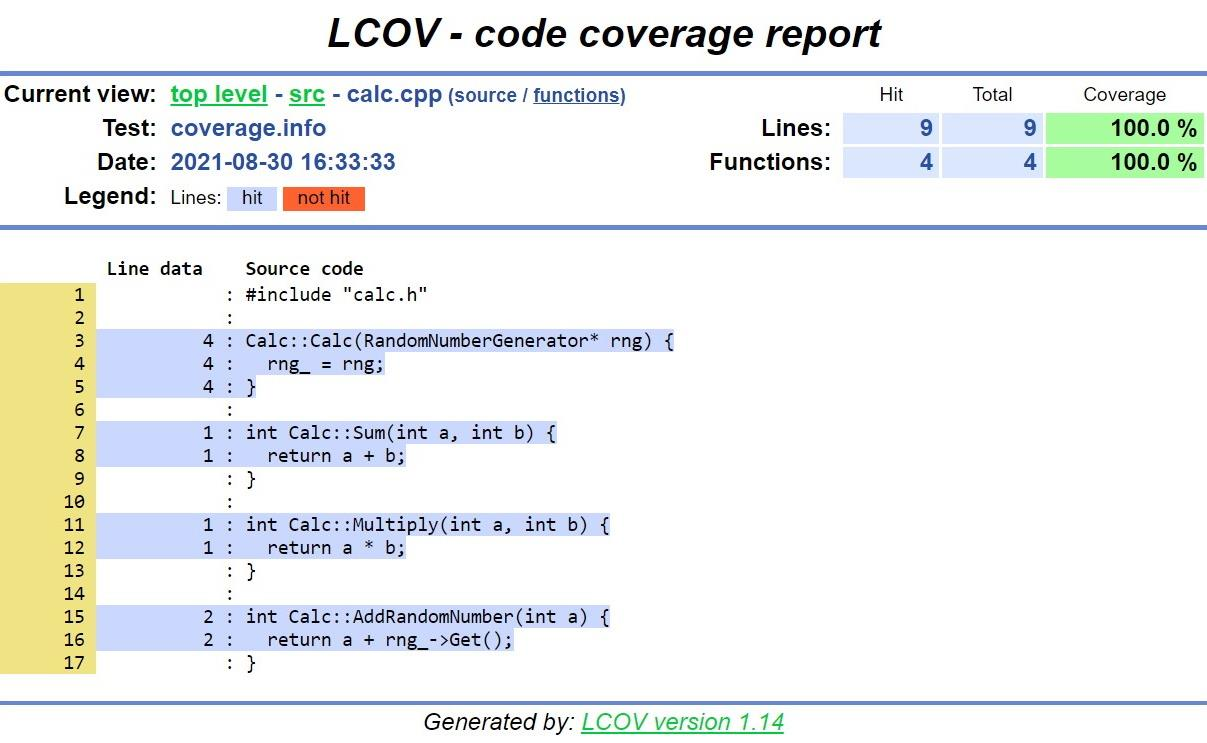
\includegraphics[width=0.8\textwidth]{content/3/chapter8/images/4.jpg}\\
图8.4 代码覆盖率报告的详细视图
\end{center}

有多种生成类似报告的方法,在不同的平台和编译器中有所不同,但通常遵循相同的过程:准备要度量的SUT,并获得基线、指标和报告。

最简单的工具叫做LCOV,是gcov的图形前端,gcov是来自GNU编译器集合(GCC)的覆盖实用程序。LCOV将生成HTML覆盖率报告,并在内部使用gcov度量覆盖率。如果您正在使用Clang,不必担心——Clang支持以这种格式生成指标。可以从Linux测试项目(\url{https://github.com/linux-test-project/lcov})维护的官方存储库中获得LCOV,或者简单地使用包管理器。它是一个针对linux的实用程序,也可以在macOS上运行它,但不支持Windows平台。最终用户通常不关心测试覆盖率,所以可以在构建环境中手动安装LCOV,而不是将其绑定到项目中。

为了衡量覆盖率,需要做以下工作:

\begin{enumerate}
\item 
Debug配置中编译,使用编译器标志启用代码覆盖。这将生成覆盖率注释(.gcno)文件。

\item 
将测试可执行文件与gcov库链接起来。

\item 
不运行测试的情况下,收集基线的覆盖率度量。

\item 
运行测试。这将创建覆盖率数据(.gcda)文件。

\item 
将指标收集到聚合的信息文件中。

\item 
生成一个(.html)报告。
\end{enumerate}

应该从解释为什么必须在Debug配置中编译代码开始。最重要的原因是,调试配置通常禁用任何带有-O0标志的优化。CMake默认在CMAKE\_CXX\_FLAGS\_DEBUG变量中这样做(在文档中没有说明这一点)。除非决定重写此变量,否则调试版本应该是未优化的。这是为了防止任何内联和其他类型的隐式代码简化。否则,将很难跟踪哪条机器指令来自哪行源代码。

首先,需要指示编译器将必要的工具添加到SUT中。要添加的确切标志是编译器特定的;然而,两个主要的编译器——gcc和clang——提供了相同的覆盖标志,支持覆盖,生成与gcc兼容的gcov格式的数据。

这就是如何将覆盖工具添加到上一节的示例SUT中:

\begin{lstlisting}[style=styleCMake]
# chapter08/06-coverage/src/CMakeLists.txt

add_library(sut STATIC calc.cpp run.cpp rng_mt19937.cpp)
target_include_directories(sut PUBLIC .)
if (CMAKE_BUILD_TYPE STREQUAL Debug)
	target_compile_options(sut PRIVATE --coverage)
	target_link_options(sut PUBLIC --coverage)
	add_custom_command(TARGET sut PRE_BUILD COMMAND
						find ${CMAKE_BINARY_DIR} -type f
						-name '*.gcda' -exec rm {} +)
endif()

add_executable(bootstrap bootstrap.cpp)
target_link_libraries(bootstrap PRIVATE sut)
\end{lstlisting}

一步步来分解:

\begin{enumerate}
\item 
确保正在使用if(STREQUAL)在Debug配置中运行。记住,除非运行带有-DCMAKE\_BUILD\_TYPE=Debug选项的cmake,否则无法获得覆盖率。

\item 
为sut库中的所有目标文件的PRIVATE编译选项添加-{}-coverage。

\item 
在PUBLIC链接器选项中添加-{}-coverage:GCC和Clang都将此解释为将gcov(或兼容的)库与所有依赖sut(由于传播属性)的目标链接起来的请求。

\item 
引入add\_custom\_command()指令清除过时的.gcda文件。添加此命令的原因将在避免SEGFAULT问题中详细讨论。
\end{enumerate}

这足以产生代码覆盖率。若正在使用诸如Clion之类的IDE,将能够在覆盖范围内运行单元测试,并在内置报告视图中获得结果。然而,这在任何可能在CI/CD中运行的自动化流水中都不起作用。为了得到报告,需要用LCOV生成报告。

为了达到这个目的,可以定义一个叫做覆盖率的新目标。为了保持整洁,可以在测试列表文件中使用的另一个文件中定义一个单独的函数AddCoverage,如下所示:

\begin{lstlisting}[style=styleCMake]
# chapter08/06-coverage/cmake/Coverage.cmake

function(AddCoverage target)
	find_program(LCOV_PATH lcov REQUIRED)
	find_program(GENHTML_PATH genhtml REQUIRED)
	
	add_custom_target(coverage
		COMMENT "Running coverage for ${target}..."
		COMMAND ${LCOV_PATH} -d . --zerocounters
		COMMAND $<TARGET_FILE:${target}>
		COMMAND ${LCOV_PATH} -d . --capture -o coverage.info
		COMMAND ${LCOV_PATH} -r coverage.info '/usr/include/*'COMMAND ${GENHTML_PATH} -o coverage filtered.info
			--legend
		COMMAND rm -rf coverage.info filtered.info
		WORKING_DIRECTORY ${CMAKE_BINARY_DIR}
		)
endfunction()
\end{lstlisting}

首先检测lcov和genhtml(来自LCOV包的两个命令行工具)的路径。REQUIRED关键字指示CMake在未找到它们时抛出错误。接下来,按照以下步骤添加一个自定义覆盖率目标:

\begin{enumerate}
\item 
清除以前运行的所有计数器。

\item 
运行目标可执行文件(使用生成器表达式获取其路径)。\$<target\_file: target>是一个异常生成器表达式,将隐式地在TARGET上添加一个依赖项,导致在执行命令之前构建。这里提供target作为该函数的参数。

\item 
在系统头文件('/usr/include/*')上删除(-r)不需要的覆盖数据,并输出到另一个文件(-o filtered.info)。

\item 
覆盖率目录中生成一个HTML报告,并添加一个-{}-legend颜色。

\item 
删除临时的.info文件。

\item 
指定WORKING\_DIRECTORY关键字将构建树设置为所有命令的工作目录。
\end{enumerate}

这些是GCC和Clang的一般步骤,要知道gcov工具的版本必须与编译器的版本匹配。换句话说,不能对clang编译的代码使用GCC的gcov工具。要将lcov指向Clang的gcov工具,可以使用-{}-gcov-tool参数。这里的问题是必须是一个单一的可执行文件。为了解决这个问题,可以提供一个简单的包装器脚本(记得用chmod +x将其标记为可执行文件):

\begin{lstlisting}[style=stylePython]
# cmake/gcov-llvm-wrapper.sh

#!/bin/bash
exec llvm-cov gcov "$@"
\end{lstlisting}

在上一个函数中对\$\{LCOV\_PATH\}的所有调用都应该获得以下标志:

\begin{lstlisting}[style=stylePython]
--gcov-tool ${CMAKE_SOURCE_DIR}/cmake/gcov-llvm-wrapper.sh
\end{lstlisting}

确保这个函数可以包含在测试列表文件中,可以在主列表文件中扩展include搜索路径:

\begin{lstlisting}[style=styleCMake]
# chapter08/06-coverage/CMakeLists.txt

cmake_minimum_required(VERSION 3.20.0)
project(Coverage CXX)
enable_testing()
list(APPEND CMAKE_MODULE_PATH "${CMAKE_SOURCE_DIR}/cmake")
add_subdirectory(src bin)
add_subdirectory(test)
\end{lstlisting}

这一小行允许在项目中包含cmake目录中的所有.cmake文件。现在可以在测试列表文件中使用Coverage.cmake,像这样:

\begin{lstlisting}[style=styleCMake]
# chapter08/06-coverage/test/CMakeLists.txt (fragment)

# ... skipped unit_tests target declaration for brevity

include(Coverage)
AddCoverage(unit_tests)

include(GoogleTest)
gtest_discover_tests(unit_tests)
\end{lstlisting}

要构建这个目标,使用以下命令(注意第一个命令以DCMAKE\_BUILD\_TYPE=Debug构建类型选择结束):

\begin{tcblisting}{commandshell={}}
# cmake -B <binary_tree> -S <source_tree>
    -DCMAKE_BUILD_TYPE=Debug
# cmake --build <binary_tree> -t coverage
\end{tcblisting}

执行上述所有步骤后,将看到如下简短的输出:

\begin{tcblisting}{commandshell={}}
Writing directory view page.
Overall coverage rate:
  lines......: 95.2% (20 of 21 lines)
  functions..: 75.0% (6 of 8 functions)
[100%] Built target coverage
\end{tcblisting}

接下来,在浏览器中打开coverage/index.html文件并欣赏报告!不过只有一个小问题……


\subsubsubsection{8.6.1\hspace{0.2cm}避免SEGFAULT问题}

开始在这样的解决方案中编辑源代码时可能会陷入麻烦。这是因为覆盖率信息分为了两部分:

\begin{itemize}
\item 
gcno文件,或GNU覆盖注释,在编译SUT期间生成

\item 
gcda文件,或GNU覆盖数据,在测试运行期间生成和更新
\end{itemize}

“更新”功能是分段错误的潜在来源。在最初运行测试之后,会留下一堆gcda文件,这些文件不会删除。若对源代码做一些更改并重新编译目标文件,就会创建新的gcno文件。然而,没有擦除步骤——旧的gcda文件仍然遵循陈旧的源文件。当执行unit\_tests二进制文件时(发生在gtest\_discover\_tests宏中),覆盖率信息文件将不匹配,将收到一个SEGFAULT(段错误)错误。

为了避免这个问题,应该删除任何过时的gcda文件。由于sut实例是一个STATIC库,可以将add\_custom\_command(TARGET)与构建事件相关。清理将在重新构建开始之前执行。

在扩展阅读部分可以找到更多信息的链接。























































